\chapter{SYSTEM DESIGN}

\section{Requirement Specification}

\subsection{Functional Requirements}

The proposed MorphAI system shall provide the following functional requirements:

\begin{itemize}
\item \textbf{Input Handling:} The system shall accept facial images from the CelebA-HQ dataset for training and evaluation.

\item \textbf{Image Pre-processing:} The system shall resize input facial images to $256 \times 256$ pixels and prepare them for the reconstruction pipeline.

\item \textbf{Facial Landmark Detection:} The system shall use MediaPipe Face Mesh to detect facial landmarks from the input image.

\item \textbf{Mask Generation:} The system shall generate facial masks for selected regions using semantic facial regions and random rectangular masks.

\item \textbf{Landmark Heatmap Generation:} The system shall convert the detected facial landmarks into a landmark heatmap to provide additional facial structure information.

\item \textbf{Model Input Preparation:} The system shall combine the three RGB channels, one binary mask channel, and one landmark heatmap channel to create a five-channel input of size $5 \times 256 \times 256$.

\item \textbf{Facial Reconstruction:} The system shall use the modified LGNet generator to reconstruct the masked facial regions and produce a $256 \times 256$ RGB facial image.

\item \textbf{Identity Preservation:} The system shall use a pretrained facial recognition model to calculate identity loss and encourage the reconstructed image to preserve the identity of the input subject.

\item \textbf{Model Training:} The system shall train the modified LGNet using a composite loss consisting of reconstruction, perceptual, style, identity, and adversarial objectives.

\item \textbf{Evaluation:} The system shall evaluate reconstructed images using image-quality and identity-based metrics, including PSNR, SSIM, LPIPS, FID, RMSE, RMSE-log, and identity similarity.

\item \textbf{Inference:} The system shall accept a facial image and generate a reconstructed facial image using the trained MorphAI model.

\item \textbf{Output:} The system shall provide the reconstructed facial image while preserving the visible facial structure and attempting to maintain the identity of the subject.
\end{itemize}

\subsection{Non-Functional Requirements}

The MorphAI system should satisfy the following non-functional requirements:

\begin{itemize}
\item \textbf{Performance:} The system should use GPU acceleration to reduce model training and inference time.

\item \textbf{Accuracy:} The system should generate realistic facial reconstructions while maintaining high structural and identity similarity.

\item \textbf{Reliability:} The preprocessing and reconstruction pipeline should produce consistent results for valid facial images and different masking conditions.

\item \textbf{Robustness:} The system should handle variations in facial expression, pose, lighting, and masked facial regions as effectively as possible.

\item \textbf{Usability:} The system should provide a simple pipeline for preparing facial images, generating reconstructions, and evaluating the results.

\item \textbf{Maintainability:} The system should use modular components for preprocessing, landmark detection, mask generation, model training, inference, and evaluation so that individual components can be modified or improved easily.

\item \textbf{Scalability:} The framework should allow future experiments with larger datasets, different facial reconstruction models, and additional identity-preservation methods.

\item \textbf{Resource Efficiency:} The system should be capable of training and testing within the available GPU and memory resources without requiring specialized 3D facial scanning hardware.
\end{itemize}
\newpage

\section{Use Case Diagram}
      The Use Case Diagram \ref{fig:use case diagram} illustrates the interaction between the user and the MorphAI Facial Appearance Transformation System.
    \begin{figure}[H]
        \centering
        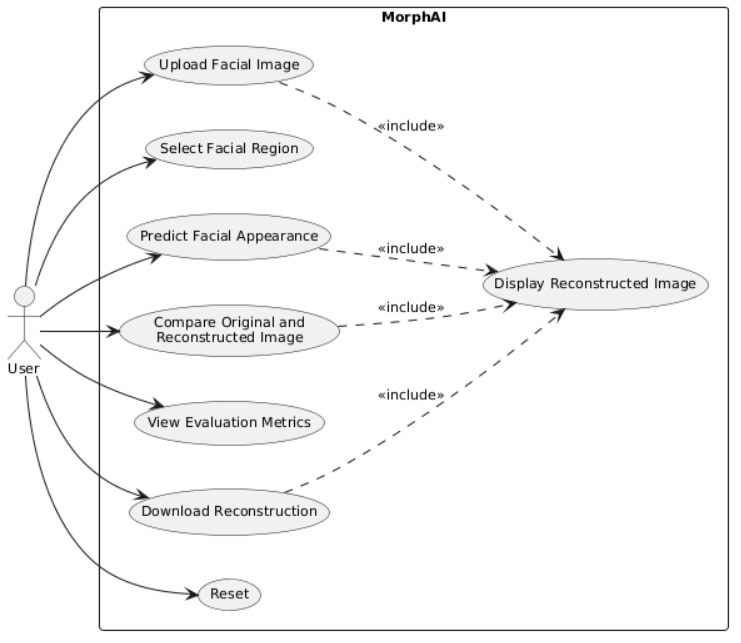
\includegraphics[scale=0.5]{img/usecase.png}
        \caption{Use Case Diagram of MorphAI}
        \label{fig:use case diagram}
   \end{figure}
     \noindent The process begins when the user uploads a facial image and selects the facial region to be reconstructed. The user can then generate a facial appearance prediction, after which the reconstructed image is displayed. The user can compare the original and reconstructed images, view evaluation metrics, download the reconstruction, or reset the prediction.
%\section{Activity Diagram}
   % \begin{figure}[H]
      %  \centering
        %\includegraphics[scale=0.69]{img/ActivityDiagram.png}
       % \caption{Activity Diagram}
       % \label{fig:activity diagram}
  % \end{figure}
 %  The activity diagram illustrates the complete workflow of the system from start to finish. The process begins when the user uploads a handwritten image. If the image format is invalid, an error message is displayed and the process terminates. If the format is valid, the image preview is shown and the image enters the preprocessing pipeline, which consists of grayscale conversion, binarization, deskewing, and tight cropping. The preprocessed image is then fed into the fine-tuned TrOCR model to generate Unicode Nepali text. The post-processing stage runs in parallel to display the recognized word, generate a character-level confidence breakdown, and produce a pipeline processing log. Finally, if the user chooses to export the result, they can either download it as a .txt file or copy it to the clipboard, after which the process ends.

\newpage
\section{Class Diagram for System}
This class diagram \ref{fig:classdiagram} illustrates the structure and
relationships among the major components of the MorphAI facial inpainting
system.

\begin{figure}[H]
    \centering
    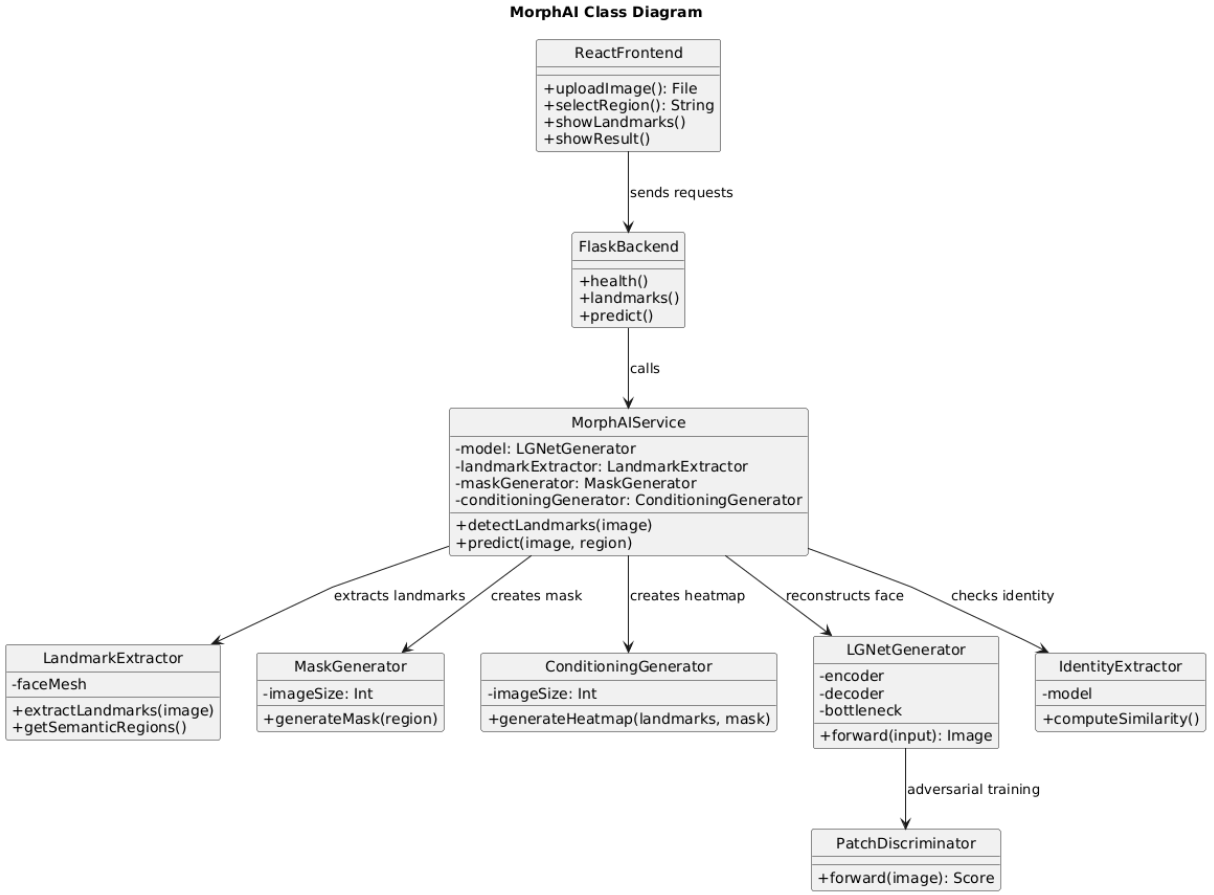
\includegraphics[scale=0.5]{img/class_diagram.png}
    \caption{Class diagram of MorphAI system}
    \label{fig:classdiagram}
\end{figure}
 \noindent The \textbf{ReactFrontend} serves as the entry point where the user uploads a facial image, selects the target facial region, and views the reconstructed result. It communicates with the \textbf{FlaskBackend}, which handles health checks, landmark extraction, and prediction requests. The \textbf{MorphAIService} coordinates the main processing components, including the \textbf{LandmarkExtractor}, \textbf{MaskGenerator}, \textbf{ConditioningGenerator}, \textbf{LGNetGenerator}, and \textbf{IdentityExtractor}. The \textbf{LandmarkExtractor} detects facial landmarks and semantic regions, while the \textbf{MaskGenerator} creates the mask for the selected facial region. The \textbf{ConditioningGenerator} uses the extracted landmarks and mask to generate the conditioning heatmap. These inputs are provided to the \textbf{LGNetGenerator}, which reconstructs the masked facial region using its encoder, decoder, and bottleneck components. The generated image is further evaluated through the \textbf{PatchDiscriminator} during adversarial training and the \textbf{IdentityExtractor} to verify identity preservation. Each component has a well-defined responsibility, providing a structured flow from facial image input and region selection to reconstructed and identity-preserving facial output.



  
%\section{Class Diagram for Data }

%\section{Database Schema}

\section{Sequence Diagram}
    \begin{figure}[H]
        \centering
        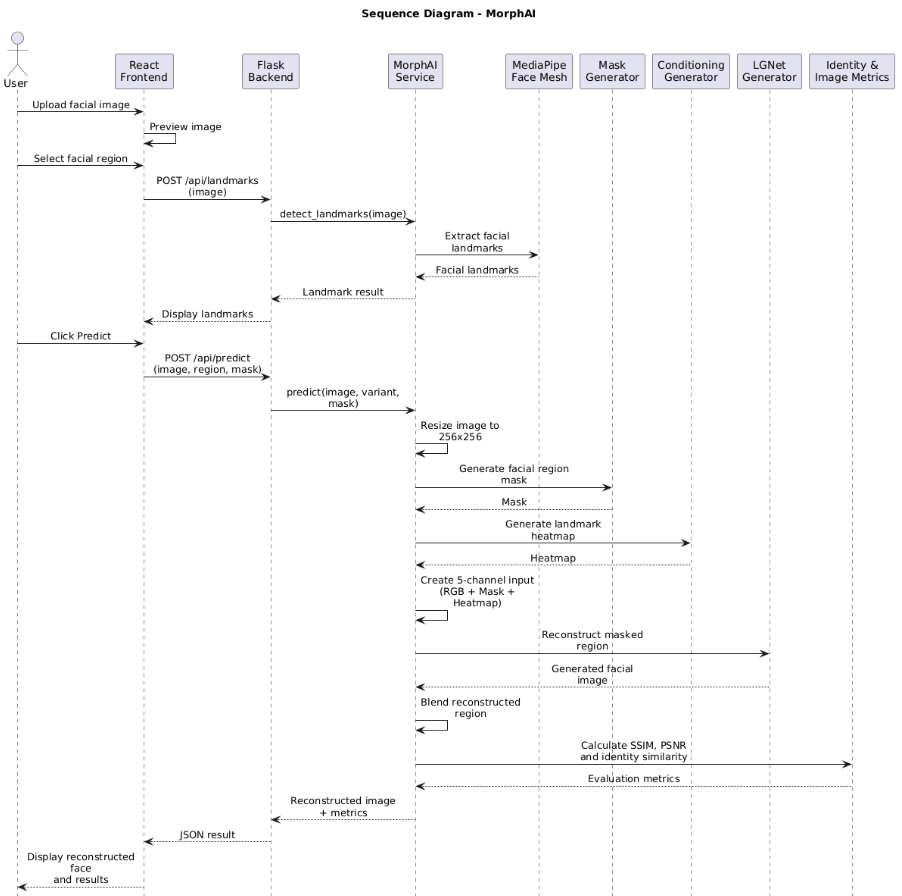
\includegraphics[scale=0.65]{img/activity_diagram.png}
        \caption{Sequence Diagram of MorphAI system}
        \label{fig:sequence diagram}
   \end{figure}

\clearpage
\noindent The sequence diagram \ref{fig:sequence diagram} illustrates the interaction between system components during facial inpainting. The user uploads an image and selects a facial region through the React frontend. The Flask backend forwards the request to the MorphAIService, which extracts landmarks, generates a mask and heatmap, and forms the five-channel input for the LGNetGenerator. The generated facial image is then returned to the frontend for display, while the IdentityExtractor evaluates identity preservation.
\newline
\noindent The backend then sends the image to the MorphAIService, which generates the facial mask, landmark heatmap, and five-channel input for the LGNetGenerator. The reconstructed image is blended and evaluated using SSIM, PSNR, and identity similarity before being returned to the frontend and displayed to the user.
   %  \begin{figure}[H]
   %      \centering
   %      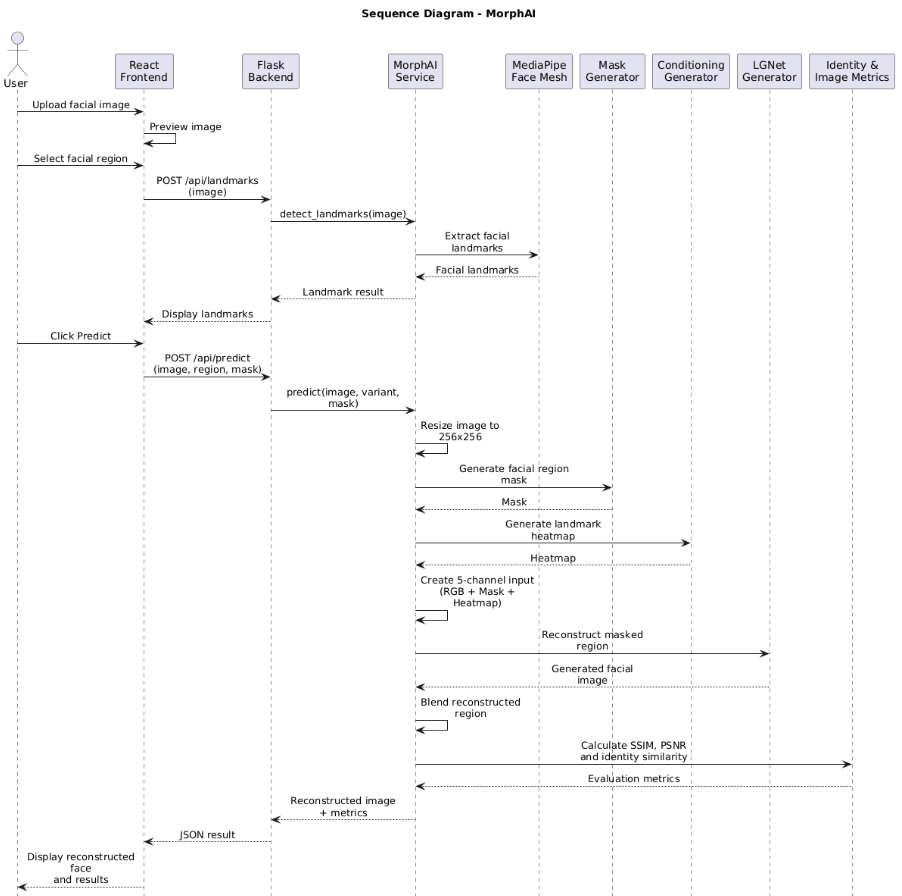
\includegraphics[scale=0.65]{img/activity_diagram.png}
   %      \caption{Sequence Diagram of MorphAI system}
   %      \label{fig:sequence diagram}
   % \end{figure}


%\section{Data Flow Diagram}

   % \begin{figure}[H]
      %  \centering
       % \includegraphics[scale=0.38]{img/dfd0.png}
       % \caption{Level 0 Data Flow Diagram}
       % \label{fig:Level 0 Data Flow Diagram}
  % \end{figure}
  % The context diagram provides a high-level overview of the system. The user provides a handwritten image as input to the Nepali Handwritten Word Recognition System. The system processes the image and returns the recognized Unicode Nepali text, downloadable output, and confidence logs back to the user. Any invalid image format triggers an error notification.

   % \begin{figure}[H]
      %  \centering
       % \includegraphics[scale=0.5]{img/Level1.jpg}
      %  \caption{Level 1 Data Flow Diagram}
       % \label{fig:Level 1 Data Flow Diagram}
   %\end{figure}
%\noindent
%The Level 1 Data Flow Diagram breaks down the internal processes of the system. The user submits a handwritten image which enters the Upload Image process. The raw image is then passed to the Preprocess Image process where it is cleaned and normalized. The cleaned image is fed into the Run TrOCR Inference process, which loads model weights from the TrOCR Model data store. The generated token IDs are passed to the Decode Output process, which references the Nepali Tokenizer data store to map tokens to Unicode characters. The resulting Unicode text is then passed to the Display Result process, which returns the recognized word and character breakdown to the user.





%\section{Deployment Diagram}
%\textbf{Note: All the diagram is not mandatory..select according to the type of project you are going to do.}